\documentclass[addpoints,answers]{exam}

\usepackage{graphicx}
\usepackage{epstopdf}
\usepackage{calc}
\usepackage{enumitem}
\usepackage{amsmath}

\begin{document}
\begin{center}
{\bf COMP406 Midterm}

\end{center}
\vspace{0.2in}
\makebox[\textwidth]{NAME:\enspace\hrulefill}

\vspace{0.2in}

\section*{Directions}
Read carefully. Work individually. Write legibly. Check work. Complete in 1 hour.
\begin{description}[leftmargin=!,labelwidth=\widthof{\bfseries Beforehand}]
\item[Beforehand] Visit the restroom if necessary. Close your laptop. Clear your desk. Silence your phone.
\item[DO] Use pencil, eraser, pen, or scratch paper to complete this exam.
\item[DO NOT] Distract others, talk, use electronic devices, notes, smoke signals, gestures, Morse code, \ldots
\item[Confused?] Assume only what is given. I may clarify, but I cannot answer: ``Is this right (or wrong)?''
\end{description}

\begin{questions}

\section{Definitions}

\question (Check all that apply) Free software is code that you can\ldots

\begin{oneparcheckboxes}
\choice run
\choice study
\choice change
\choice distribute
\choice sell
\end{oneparcheckboxes}

\section{People}
\uplevel{Match accomplishments to the person.

\begin{oneparchoices}
\choice Bruce Perens % A
\choice Eric Raymond % B
\choice Linus Torvalds % C
\choice Mark Shuttleworth % D
\choice Michael Tiemann % E
\choice Richard Stallman % F
\choice N/A
\end{oneparchoices}
}

\question Billionaire who went to space and started Ubuntu, among other things. \answerline[D]
\question Entrepreneur and contributor to \verb$g++$. \answerline[E]
\question MacArthur Fellowship (Genius Grant) Awardee and FSF founder, among other things. \answerline[F]
\question Finn who wrote the initial version of \verb$git$, among other things. \answerline[C]
\question Amateur radio enthusiast who wrote BusyBox and \emph{The Open Source Definition}. \answerline[A]
\question Libertarian and author of \emph{The Cathedral and the Bazaar}. \answerline[B]
\pagebreak

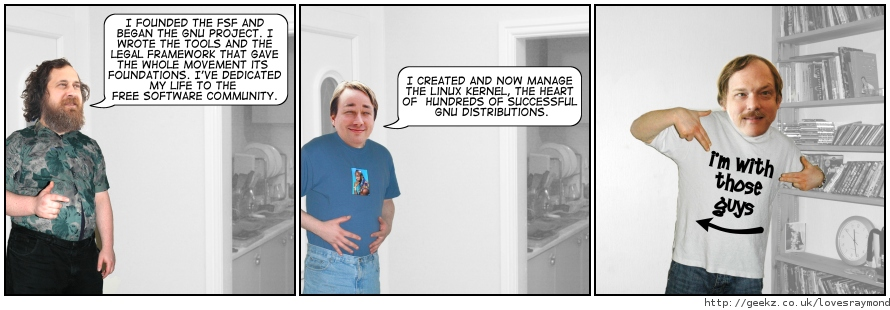
\includegraphics[width=5.5in]{people.jpg}

\section{Licensing}

\uplevel{Match project descriptions to one of these categories by completing this sentence: ``The code is \ldots'' Choose the most specific category if more than one category is relevant.

\begin{oneparchoices}
\choice Copyrighted % A
\choice Copylefted % B
\choice Permissively-licensed % C
\choice Pirated % D
\choice Proprietary % E
\choice Public domain % F
\end{oneparchoices}
}

\question A project in which the authors have waived all copyrights. \answerline[F]
\question A project provides binary downloads, but no source code. \answerline[E]
\question The project misrepresents authorship, license terms, or both. \answerline[D]

\question The project license allows users to run it, study it, make copies and changes, but distribution of changes must be under the same license. \answerline[B]
\question Github hosts a project's source code publicly, but no license is given. \answerline[A]
\question The project license allows users to run it, study it, make copies and changes to the code and license itself. \answerline[C]

\section{Version control}

Match version control terms with the definitions.

\begin{oneparchoices}
\choice branch
\choice commit
\choice fetch
\choice merge
\choice push
\choice remote
\choice repository
\choice staging area
\choice working directory
\end{oneparchoices}

\question A timeline of changes\answerline[A]
\question A snapshot that includes author, timestamp, changes, and links to previous snapshots\answerline[B]
\question The folder with the current version\answerline[I]
\question All project history\answerline[G]
\question Receive changes\answerline[C]
\question A place to build the next snapshot\answerline[H]
\question The default is master\answerline[A]
\question A repository with a nickname and URL\answerline[F]
\question The default is origin\answerline[F]
\question Submit changes\answerline[E]
\question Weaving multiple timelines together\answerline[D]

\question In centralized version control systems (e.g., Subvesion, CVS)\ldots

\begin{choices}
\choice every developer has their own repository
\choice developers can fetch from multiple remotes
\choice typically, commit access is limited to a small, trusted group
\choice developers on a team can push without being forced to merge
\choice branches and merges are commonplace
\choice recording changes is decoupled from pushing changes
\end{choices}

\answerline[C]

\end{questions}

Each answer is worth $4$ points. Check your work. See you Monday!

\end{document}